\documentclass[conference]{IEEEtran}
\IEEEoverridecommandlockouts
\usepackage[T1]{fontenc}
\usepackage{cite}
\usepackage{amsmath,amssymb}
\usepackage{graphicx}
\usepackage{booktabs}
\usepackage{multirow}
\usepackage{array}
\usepackage{xcolor}
\usepackage{tikz}
\usetikzlibrary{arrows.meta,positioning}
\usepackage{pgfplots}
\pgfplotsset{compat=1.17}
\usepackage[hidelinks]{hyperref}

\definecolor{arch}{HTML}{E0452B}
\definecolor{data}{HTML}{E8A23A}
\definecolor{evalc}{HTML}{8A8FA3}
\definecolor{ink}{HTML}{1E2128}

\newcommand{\ex}[1]{\textit{``#1''}}

\begin{document}

\title{Build-Break Sentiment Lab: Diagnosing \emph{Why} Sentiment Classifiers Fail Under Small Stress Edits}

\author{\IEEEauthorblockN{Vaiditya Tanwar}
\IEEEauthorblockA{Natural Language Processing Course Project\\
Industry Track, Milestone M6 (Final Delivery)}
\and
\IEEEauthorblockN{Yashi Gupta}
\IEEEauthorblockA{Natural Language Processing Course Project\\
Industry Track, Milestone M6 (Final Delivery)}}

\maketitle

\begin{abstract}
Sentiment classifiers that score above 90\% on a benchmark can still flip their answer when a
sentence gains a \ex{not}, a sarcastic frame, a typo or new slang. Accuracy alone also does not
say \emph{why} a model failed, so a team cannot tell whether it needs a different model family,
more data, or a better test. We present Build-Break Sentiment Lab, a working tool that takes any
sentence, generates five deterministic stress variants (negation, synonym swap, sarcasm, typo and
out-of-vocabulary slang), runs four models drawn from four NLP paradigms (a rule-based lexicon,
Naive Bayes, averaged Word2Vec and DistilBERT) side by side, and labels each wrong prediction as
\emph{Architectural}, \emph{Data-driven} or \emph{Evaluation}. On SST-2, clean accuracy rises from
56.3\% (rule-based) to 91.1\% (BERT), yet every model collapses under inserted negation
($\leq$46.5\%) and sarcasm ($\leq$41.0\%). BERT makes zero Architectural errors: 75\% of its
failures are Data-driven and the rest come from doubtful tests. Across all models, 24\% of the
1{,}770 failures are attributed to the test rather than the model. A targeted fix for the
bag-of-words baselines (bigrams, a negation window) adds 1.4 points of accuracy but only 2.5 points
on negation, supporting the view that negation scope is an architectural limit of these models.
The prototype answers a full request (24 predictions) in 0.11--0.18\,s on a laptop.
\end{abstract}

\begin{IEEEkeywords}
sentiment analysis, robustness, behavioral testing, error analysis, negation, sarcasm, BERT, Naive Bayes, Word2Vec
\end{IEEEkeywords}

% =====================================================================
\section{Introduction}
Companies run sentiment models over product reviews, support tickets and social posts, and the
outputs feed dashboards that drive product and staffing decisions. Such models are usually chosen
by their accuracy on a held-out benchmark. That number hides \emph{how} a model breaks. A model can
score 91\% on SST-2 and still read \ex{Oh sure, the movie was great. Yeah, right.} as positive with
full confidence, as all four of our models do. When a failure like this reaches production, the
team also needs to know what to do about it: switch to a model family that can represent the
input, collect training data that covers it, or admit that the test case itself was ambiguous.

This project builds a tool for that decision. Its contributions are:
\begin{enumerate}
  \item A deterministic generator of five stress variants per sentence, with an expected label for
        each variant (Section~\ref{sec:method}).
  \item A three-way failure taxonomy (Architectural, Data-driven, Evaluation) with transparent rules
        that attach a category and a plain-language reason to every wrong prediction. The
        Evaluation category makes \emph{doubtful tests} a first-class outcome rather than hiding
        them inside model error.
  \item A controlled comparison of four paradigms from the course in one harness, on the same
        1{,}024 inputs, with accuracy, robustness and failure-category results
        (Section~\ref{sec:results}).
  \item An improvement iteration that tests whether local patches fix the largest Architectural
        failure (Section~\ref{sec:improve}).
  \item A deployed Streamlit prototype with measured latency, failure handling and a monitoring
        plan (Section~\ref{sec:deploy}).
\end{enumerate}

Section~\ref{sec:lit} reviews related work and states the gap we address.
Section~\ref{sec:problem} defines the business problem and success metrics,
Section~\ref{sec:data} describes the data, and Sections~\ref{sec:method}--\ref{sec:deploy} cover
the method, experiments, results, error analysis and deployment. We close with the separation of
reused and original work, limitations and future work.

% =====================================================================
\section{Literature Review}\label{sec:lit}

\subsection{Lexicon and rule-based sentiment}
Early opinion mining scored text with hand-built lexicons of positive and negative words. Hu and
Liu~\cite{hu2004} built an opinion lexicon to summarise customer reviews by product feature.
VADER~\cite{hutto2014} extended the lexicon approach with heuristics for negation, intensifiers,
capitalisation and punctuation, tuned for social media. Liu's survey~\cite{liu2012} covers the
family. These systems are transparent and need no training data, but their coverage is fixed by
the lexicon, and every linguistic phenomenon (negation, contrast, sarcasm) needs its own rule.
Our rule-based model is deliberately minimal (a 48-word lexicon, no negation rule) so that its
failures show what the later paradigms add.

\subsection{Statistical bag-of-words classifiers}
Pang \emph{et al.}~\cite{pang2002} showed that Naive Bayes, maximum entropy and SVM classifiers on
bag-of-words features beat human-written keyword baselines on movie reviews, and that sentiment is
harder than topic classification. They also tried tagging words after a negator, an early local
fix for negation. Wang and Manning~\cite{wang2012} found that word bigrams consistently help
sentiment classification and that Naive Bayes is a strong baseline on short snippets. Our
improvement iteration re-tests these two ideas (bigrams, a local negation window) specifically
against negation robustness. Councill \emph{et al.}~\cite{councill2010} and the survey by
Wiegand \emph{et al.}~\cite{wiegand2010} show that detecting the \emph{scope} of a negation matters
more than detecting the negator, which local features cannot do.

\subsection{Distributional embeddings}
Word2Vec~\cite{mikolov2013a,mikolov2013b} learns dense word vectors from co-occurrence. A common
sentence representation is the mean of the word vectors, which discards word order. Iyyer
\emph{et al.}~\cite{iyyer2015} showed that such unordered averaging, followed by deep layers, can
rival syntactic models on sentiment, while its errors concentrate on negation and contrastive
constructions. Our Word2Vec model uses the plain average with a logistic-regression head, trained
only on SST-2, which tests how far order-free embeddings go with in-domain data alone.

\subsection{Compositional and pretrained transformer models}
The Stanford Sentiment Treebank~\cite{socher2013} labelled every phrase of a parse tree so that a
recursive network could learn how negation and contrast compose; SST-2 is its binary version and
is part of GLUE~\cite{wang2019glue}. BERT~\cite{devlin2019} pretrains a bidirectional transformer
and fine-tunes it per task; DistilBERT~\cite{sanh2019} distils it into a model about 40\% smaller
and 60\% faster that keeps most of its accuracy. Transformers read the full word order, so in
principle they can represent negation scope and sarcastic framing.

\subsection{Robustness and behavioural testing}
Held-out accuracy overestimates real-world performance. Jia and Liang~\cite{jia2017} broke reading
comprehension systems with distracting sentences, and Belinkov and Bisk~\cite{belinkov2018} showed
that synthetic and natural character noise breaks neural translation. CheckList~\cite{ribeiro2020}
organises testing by capability with minimum-functionality, invariance and directional tests, and
found serious negation failures in commercial and BERT-based sentiment models. Contrast
sets~\cite{gardner2020} and counterfactually augmented data~\cite{kaushik2020} use minimal human
edits that flip the label, and TextAttack~\cite{morris2020} automates perturbation attacks. On the
evaluation side, Gururangan \emph{et al.}~\cite{gururangan2018} showed that annotation artefacts can
make a benchmark measure the wrong thing.

\subsection{Negation and sarcasm}
Ettinger~\cite{ettinger2020} and Kassner and Sch\"utze~\cite{kassner2020} found that pretrained
language models are largely insensitive to negation in cloze-style probes, and Hossain
\emph{et al.}~\cite{hossain2020} showed that NLI benchmarks contain few negations that matter.
Sarcasm often pairs positive words with a negative situation~\cite{riloff2013}, and detecting it
is treated as a separate task~\cite{joshi2017}. Both phenomena are rare in SST-2, which predicts
that even BERT will be weak on them.

\subsection{Structured comparison and research gap}
Table~\ref{tab:lit} compares the works closest to ours. Prior robustness work reports \emph{whether}
a model passes a test, usually for one model family at a time. It rarely says \emph{why} each
failure happened in terms a team can act on, and it treats the expected label of a perturbed
input as ground truth. The gap we address is \textbf{per-failure attribution across paradigms}:
one harness that runs symbolic, statistical, distributional and pretrained models on the same
edits and labels each failure with the fix it implies, including the case where the test is at
fault.

\begin{table*}[t]
\centering
\caption{Structured comparison of related work}
\label{tab:lit}
\footnotesize
\begin{tabular}{@{}p{3.0cm}p{2.6cm}p{2.5cm}p{3.6cm}p{4.6cm}@{}}
\toprule
\textbf{Work} & \textbf{Paradigm} & \textbf{Data} & \textbf{Main finding} & \textbf{Limitation relative to our goal} \\
\midrule
Hu \& Liu 2004~\cite{hu2004} & Lexicon & Product reviews & Lexicons summarise opinions per feature & Fixed coverage; no robustness analysis \\
VADER 2014~\cite{hutto2014} & Lexicon + rules & Social media & Rules for negation and intensity work well on social media text & One paradigm; failures not categorised \\
Pang \emph{et al.} 2002~\cite{pang2002} & Bag of words (NB, SVM) & Movie reviews & ML beats keyword baselines; sentiment harder than topic & Accuracy only; negation tagging is local \\
Wang \& Manning 2012~\cite{wang2012} & NB / NBSVM + bigrams & Several sentiment sets & Bigrams help; NB strong on snippets & No stress tests of negation scope \\
Socher \emph{et al.} 2013~\cite{socher2013} & Recursive network & SST & Phrase-level labels capture composition & Clean accuracy; no perturbation study \\
Iyyer \emph{et al.} 2015~\cite{iyyer2015} & Averaged embeddings & SST, IMDB & Unordered averaging rivals syntax & Order loss noted, not quantified per edit \\
DistilBERT 2019~\cite{sanh2019} & Pretrained transformer & GLUE & Smaller, faster, near-BERT accuracy & No robustness evaluation \\
CheckList 2020~\cite{ribeiro2020} & Behavioural testing & Sentiment, QA, QQP & Many capability failures, incl.\ negation & Pass/fail rates; no cause per failure; tests assumed correct \\
Ettinger 2020~\cite{ettinger2020} & Probing BERT & Psycholinguistic sets & BERT insensitive to negation & Language modelling, not classification \\
Kaushik \emph{et al.} 2020~\cite{kaushik2020} & Counterfactual data & IMDB & Minimal edits expose spurious cues & Human edits are costly; one model family \\
\midrule
\textbf{This work} & All four paradigms & SST-2 & BERT: 0 Architectural failures; 24\% of all failures are doubtful tests & Template edits; rule-based labels (Section~\ref{sec:limits}) \\
\bottomrule
\end{tabular}
\end{table*}

% =====================================================================
\section{Problem Definition and Business Case}\label{sec:problem}

\textbf{Problem.} A team must choose and monitor a sentiment model without knowing where it breaks
or why. \textbf{Users.} (i) ML and data engineers choosing a model before deployment; (ii) product
and customer-experience analysts who need to know which inputs to distrust on a dashboard; (iii)
NLP students comparing classic and modern methods on their own sentences.

\textbf{Business objective.} Reduce the cost of shipping a fragile sentiment model by finding
robustness failures before deployment and routing each to the right fix: Architectural $\rightarrow$
change model family; Data-driven $\rightarrow$ add training data; Evaluation $\rightarrow$ fix the
test or its label.

\textbf{Success metrics.} Table~\ref{tab:metrics} lists the targets fixed in Milestone M1 and the
measured outcome. \textbf{Feasibility.} SST-2 is public, all training fits on a laptop, and BERT is
used as a pretrained checkpoint, so no labelled data collection or GPU cluster is needed.

\begin{table}[t]
\centering
\caption{Success metrics: target vs.\ measured}
\label{tab:metrics}
\footnotesize
\begin{tabular}{@{}p{3.6cm}p{1.8cm}p{2.1cm}@{}}
\toprule
\textbf{Metric} & \textbf{Target} & \textbf{Measured} \\
\midrule
Best model accuracy, SST-2 val. & $\geq$ 0.85 & 0.911 (BERT) \\
Variants per sentence & 5, deterministic & 4--5$^{a}$ \\
Latency, one full request & $<$ 2\,s & 0.11--0.18\,s \\
Failures with category + reason & 100\% & 100\% \\
Agreement with a human reviewer & $\geq$ 80\% on 50 & not measured \\
\bottomrule
\multicolumn{3}{@{}p{7.7cm}@{}}{\scriptsize $^{a}$The synonym edit is skipped when no listed word occurs.}
\end{tabular}
\end{table}

% =====================================================================
\section{Data}\label{sec:data}

\subsection{Source and splits}
We use SST-2~\cite{socher2013} as distributed in GLUE~\cite{wang2019glue}: English snippets of
Rotten Tomatoes reviews~\cite{pang2005}, labelled positive or negative. GLUE test labels are hidden,
so the 872-sentence validation split is our held-out test set. Nothing is tuned on it: the trained
models use library defaults, and the BERT checkpoint is used as released. Table~\ref{tab:splits}
gives the splits.

\begin{table}[t]
\centering
\caption{SST-2 splits and use}
\label{tab:splits}
\footnotesize
\begin{tabular}{@{}lrrl@{}}
\toprule
\textbf{Split} & \textbf{Size} & \textbf{Positive} & \textbf{Use} \\
\midrule
Train & 67{,}349 & 55.8\% & trains NB and Word2Vec \\
Validation & 872 & 50.9\% & held-out test set \\
Test & 1{,}821 & hidden & not used \\
\bottomrule
\end{tabular}
\end{table}

\subsection{Exploratory and statistical analysis}
Training items are mostly short phrases (mean 8.9 tokens, median 6, and 28.4\% have three tokens
or fewer), while validation items are full sentences (mean 17.7, median 17, 0.7\% with three
tokens or fewer). Negation words (\emph{not, no, never, n't}) appear in 13.0\% of negative and
4.9\% of positive training items but in 24.3\% and 13.5\% of validation sentences, roughly twice
as often. The most frequent negative-class words include \emph{n't} and \emph{not}, but both also
rank in the top twenty positive words, so a bag-of-words model cannot treat them as purely
negative cues. Always predicting ``positive'' scores 50.9\% on validation.

\subsection{Cleaning, leakage and privacy}
No items are removed or relabelled. Each model applies only its own light normalisation
(lowercasing and a word regex; scikit-learn defaults for Naive Bayes; WordPiece for BERT). There
are 371 duplicates within train (0.55\%), which we keep, and \textbf{0 of 872} validation sentences
appear in train, so there is no exact leakage. 5.82\% of validation tokens are out of the Naive
Bayes vocabulary. The data is public critic prose with no personal data, and the app processes
typed sentences in memory without storing or logging them. A full data card is in the repository
(\texttt{docs/02\_data\_card.md}), following the spirit of datasheets~\cite{gebru2021}.

% =====================================================================
\section{Methodology}\label{sec:method}

Fig.~\ref{fig:pipeline} shows the pipeline. One sentence and its label produce six inputs (the
original plus five variants); each goes through four models, giving 24 predictions, and every wrong
prediction is labelled.

\begin{figure}[t]
\centering
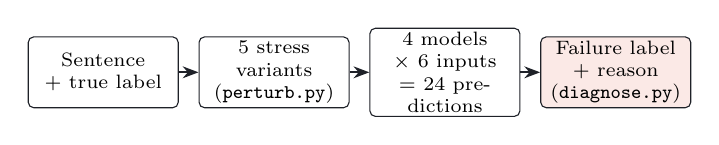
\begin{tikzpicture}[
  box/.style={draw=ink, rounded corners=2pt, align=center, font=\scriptsize, minimum height=0.9cm, text width=1.8cm, inner sep=1.5pt},
  arr/.style={-{Stealth[length=2mm]}, thick, ink}]
\node[box] (in) {Sentence\\+ true label};
\node[box, right=0.25cm of in] (pert) {5 stress\\variants\\(\texttt{perturb.py})};
\node[box, right=0.25cm of pert] (mods) {4 models\\$\times$ 6 inputs\\= 24 predictions};
\node[box, right=0.25cm of mods, fill=arch!12] (diag) {Failure label\\+ reason\\(\texttt{diagnose.py})};
\draw[arr] (in) -- (pert); \draw[arr] (pert) -- (mods); \draw[arr] (mods) -- (diag);
\end{tikzpicture}
\caption{Build-break pipeline. The same code runs interactively in the app and in batch over SST-2 (\texttt{evaluate.py}).}
\label{fig:pipeline}
\end{figure}

\subsection{Models}
All four models share one interface, \texttt{predict(text)} $\rightarrow$ (label, confidence).
\begin{itemize}
  \item \textbf{Rule-based (B0, symbolic).} 24 positive and 24 negative hand-picked words; the class
        with more matches wins, ties return positive with confidence 0.5. No negation handling.
  \item \textbf{Naive Bayes (B1, statistical).} \texttt{CountVectorizer} unigrams with
        \texttt{MultinomialNB}~\cite{pedregosa2011}, trained on SST-2 train.
  \item \textbf{Word2Vec (avg) (C1, distributional).} 100-dimensional CBOW vectors (gensim defaults)
        trained with gensim~\cite{rehurek2010} on SST-2 train (\texttt{min\_count}=1, 10 epochs,
        fixed seed); a sentence is the mean of its known word vectors, classified by logistic
        regression. Sentences with no known word return positive with confidence 0.5.
  \item \textbf{BERT (C2, pretrained transformer).} The Hugging Face~\cite{wolf2020} checkpoint
        \texttt{distilbert-base-uncased-}\allowbreak\texttt{finetuned-sst-2-english}~\cite{sanh2019}, used without
        further training, with truncation at 512 tokens.
\end{itemize}
B0 and B1 are the baselines; C1 and C2 are the candidate approaches.

\subsection{Stress variants}
\texttt{perturb.py} generates the variants with fixed rules, so the same sentence always yields the
same variants (Table~\ref{tab:variants}). Negation inserts \ex{not} after the first auxiliary verb,
removes an existing \ex{not} instead of stacking \ex{not not}, and otherwise prefixes \ex{It is not
true that}. The synonym and slang edits replace the first word found in a small table; if no slang
word matches, \ex{fr fr} is appended. The typo swaps two adjacent letters in the longest word.

\begin{table}[t]
\centering
\caption{Stress variants for \ex{The movie was great} (positive)}
\label{tab:variants}
\footnotesize
\begin{tabular}{@{}lp{4.1cm}l@{}}
\toprule
\textbf{Kind} & \textbf{Variant} & \textbf{Expected} \\
\midrule
Negation & The movie was \textbf{not} great & flipped \\
Synonym & The movie was \textbf{terrific} & same \\
Sarcasm & \textbf{Oh sure,} the movie was great\textbf{. Yeah, right.} & negative \\
Typo & The \textbf{mvoie} was great & same \\
Slang (OOV) & The movie was \textbf{bussin} & same \\
\bottomrule
\end{tabular}
\end{table}

\subsection{Failure taxonomy}
\texttt{diagnose.py} checks three groups of rules in order and returns the first match together
with a sentence explaining it.
\begin{enumerate}
  \item \textbf{Evaluation} (the test is doubtful): a \ex{not} inserted into a multi-clause sentence
        (comma, semicolon, \emph{and, but, although, though, while}), which leaves mixed sentiment;
        sarcasm wrapped around an already negative sentence; or every model failing a
        meaning-preserving edit (synonym, typo, slang), which suggests the edit changed the meaning.
  \item \textbf{Architectural} (the design cannot represent the edit): an order-insensitive model
        (rule-based, Naive Bayes, averaged Word2Vec) meets negation or sarcasm, or any input that
        contains a negation word.
  \item \textbf{Data-driven} (the design could, the data did not): the changed word is outside the
        model's vocabulary or lexicon, sarcasm for an order-aware model, or a known-word input where
        the learned association is weak or wrong.
\end{enumerate}
By construction BERT, the only order-aware model, cannot receive the Architectural label; the
interesting question is how its failures split between the other two.

\subsection{Improvement iteration}\label{sec:improve-method}
The largest Architectural failure for the baselines is negation. We therefore test the hypothesis
\textbf{H1}: \emph{giving bag-of-words models a local view of negation raises their negation
accuracy}. Two candidates follow prior work~\cite{pang2002,wang2012}: Naive Bayes with unigrams and
bigrams (\texttt{ngram\_range}=(1,2)), and the rule-based model with a negation window that flips a
lexicon word's polarity when a negator occurs in the three preceding tokens.

% =====================================================================
\section{Experimental Setup}\label{sec:setup}
\textbf{Clean accuracy} is measured on all 872 validation sentences. \textbf{Robustness} uses the
first 200 validation sentences and their variants: 200 originals and 200 each of negation, sarcasm,
typo and slang, plus 24 synonym variants (only 24 sentences contain a listed word), i.e.\ 1{,}024
inputs and 4{,}096 predictions. Accuracy per variant kind is the share of predictions equal to the
expected label. \textbf{Failure categories} are counted over every wrong prediction in the same run,
including errors on the unedited originals. \textbf{Latency} is the median and 95th percentile over
200 single-sentence calls after warm-up.

All runs are deterministic (fixed seeds, rule-based variants, no sampling) and were executed on an
Apple Silicon laptop (arm64) with PyTorch 2.15, BERT on the MPS GPU. Each experiment maps to a
script in the repository (\texttt{train.py}, \texttt{evaluate.py}, \texttt{improve.py},
\texttt{benchmark.py}, \texttt{eda.py}); outputs are saved under \texttt{results/} and an
experiment log is kept in \texttt{docs/03\_experiment\_log.md}.

% =====================================================================
\section{Results}\label{sec:results}

\subsection{Clean accuracy}
On the 872 validation sentences the rule-based model scores 0.563, Naive Bayes 0.806, averaged
Word2Vec 0.712 and BERT 0.911. Accuracy rises with each paradigm except Word2Vec, which loses to
Naive Bayes by 9.4 points.

\subsection{Robustness}
Table~\ref{tab:robust} reports accuracy per variant. Typos and slang barely matter for the trained
models (BERT drops at most 1.5 points), because most edits leave enough other sentiment words in
long sentences. Synonym accuracy is higher still, but it is measured on only 24 sentences. Negation and sarcasm break every model. BERT falls from
0.910 to 0.320 under negation and to 0.390 under sarcasm; the rule-based model scores 0.040 on
sarcasm because the frame adds no lexicon words, so the original words or a tie (which defaults to
positive) decide the answer.

\begin{table}[t]
\centering
\caption{Accuracy on 200 SST-2 validation sentences and their variants}
\label{tab:robust}
\footnotesize
\setlength{\tabcolsep}{3.5pt}
\begin{tabular}{@{}lcccccc@{}}
\toprule
\textbf{Model} & \textbf{orig.} & \textbf{neg.} & \textbf{syn.}$^{a}$ & \textbf{sarc.} & \textbf{typo} & \textbf{oov} \\
\midrule
Rule-based     & 0.535 & 0.465 & 0.708 & \textbf{0.040} & 0.530 & 0.525 \\
Naive Bayes    & 0.790 & \textbf{0.220} & 0.792 & 0.355 & 0.780 & 0.790 \\
Word2Vec (avg) & 0.685 & 0.335 & 0.792 & 0.410 & 0.690 & 0.675 \\
BERT           & 0.910 & 0.320 & 0.958 & 0.390 & 0.900 & 0.895 \\
\bottomrule
\multicolumn{7}{@{}l@{}}{\scriptsize $^{a}$24 sentences only.}
\end{tabular}
\end{table}

\subsection{Failure categories}
Fig.~\ref{fig:fail} shows the failure mix. The three order-insensitive models are dominated by
Architectural failures (203--246 each). BERT has none: 239 of its 318 failures (75\%) are
Data-driven and 79 are Evaluation. Across all models, 428 of the 1{,}770 failures (24\%) are
attributed to doubtful tests.

\begin{figure}[t]
\centering
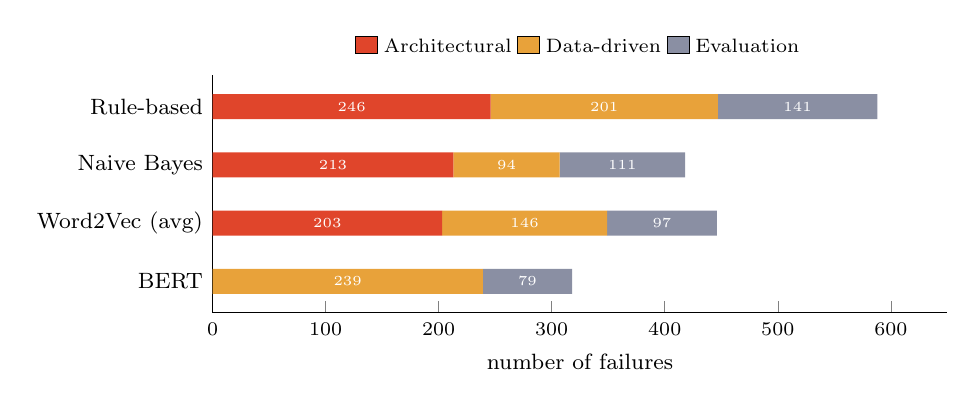
\begin{tikzpicture}
\begin{axis}[
  xbar stacked, width=0.9\columnwidth, height=4.6cm, bar width=9pt,
  xmin=0, xmax=650, xlabel={\footnotesize number of failures},
  symbolic y coords={BERT,W2V,NB,Rule}, ytick={BERT,W2V,NB,Rule}, yticklabels={BERT,Word2Vec (avg),Naive Bayes,Rule-based},
  y tick label style={font=\footnotesize}, x tick label style={font=\scriptsize},
  legend style={at={(0.5,1.03)}, anchor=south, legend columns=3, font=\scriptsize, draw=none},
  nodes near coords={\pgfmathfloatifflags{\pgfplotspointmeta}{0}{}{\pgfmathprintnumber{\pgfplotspointmeta}}},
  nodes near coords style={font=\tiny, white}, axis lines*=left, enlarge y limits=0.18]
\addplot[fill=arch, draw=none] coordinates {(246,Rule) (213,NB) (203,W2V) (0,BERT)};
\addplot[fill=data, draw=none] coordinates {(201,Rule) (94,NB) (146,W2V) (239,BERT)};
\addplot[fill=evalc, draw=none] coordinates {(141,Rule) (111,NB) (97,W2V) (79,BERT)};
\legend{Architectural, Data-driven, Evaluation}
\end{axis}
\end{tikzpicture}
\caption{Failures by category on the same 200-sentence run. BERT has no Architectural failures.}
\label{fig:fail}
\end{figure}

\subsection{Improvement iteration}\label{sec:improve}
Table~\ref{tab:improve} compares each baseline with its patched version. Bigrams raise Naive Bayes
full-validation accuracy by 1.4 points (0.806 $\rightarrow$ 0.820) and help synonyms (+4.1) and
sarcasm (+3.5), but negation improves by only 2.5 points to 0.245, and the unedited originals,
typos and slang get worse by 3.0--4.0 points. The negation window moves the rule-based model by 0.5
points overall and 1.0 point on negation. \textbf{H1 is not supported in any practical sense}:
negation accuracy stays far below chance for Naive Bayes and below 0.5 for both models. Local
features cannot reach the scope of a negation in a long, multi-clause sentence, which supports the
Architectural label for these failures.

\begin{table}[t]
\centering
\caption{Improvement iteration (accuracy)}
\label{tab:improve}
\footnotesize
\setlength{\tabcolsep}{3pt}
\begin{tabular}{@{}lccccc@{}}
\toprule
\textbf{Model} & \textbf{full val} & \textbf{orig.} & \textbf{neg.} & \textbf{sarc.} & \textbf{typo} \\
\midrule
Naive Bayes           & 0.806 & 0.790 & 0.220 & 0.355 & 0.780 \\
\quad + bigrams       & \textbf{0.820} & 0.760 & 0.245 & 0.390 & 0.740 \\
Rule-based            & 0.563 & 0.535 & 0.465 & 0.040 & 0.530 \\
\quad + neg.\ window  & \textbf{0.568} & 0.545 & 0.475 & 0.050 & 0.540 \\
\bottomrule
\end{tabular}
\end{table}

% =====================================================================
\section{Error Analysis}\label{sec:error}
Table~\ref{tab:cases} lists representative failures taken from the app, with the category and the
reason the rules attach.

\begin{table}[t]
\centering
\caption{Representative failures}
\label{tab:cases}
\footnotesize
\begin{tabular}{@{}p{2.6cm}p{1.35cm}p{1.15cm}p{2.0cm}@{}}
\toprule
\textbf{Input} & \textbf{Model $\rightarrow$ pred.} & \textbf{Category} & \textbf{Reason} \\
\midrule
The movie was not great & Rule $\rightarrow$ pos. & Arch. & counts \emph{great}, cannot see \emph{not} \\
The movie was bussin & NB $\rightarrow$ neg. & Data & \emph{bussin} never seen in training \\
I despised the ending & Rule $\rightarrow$ pos.\ (tie) & Data & \emph{despised} not in lexicon \\
Oh sure, the movie was great. Yeah, right. & BERT $\rightarrow$ pos.\ (1.00) & Data & SST-2 has almost no sarcasm \\
The movie was not great and the acting was good & all four $\rightarrow$ pos. & Eval. & mixed; ``negative'' label doubtful \\
\bottomrule
\end{tabular}
\end{table}

Three patterns explain most errors. \textbf{(1) Order blindness.} For the three older models,
\emph{not great} and \emph{great} differ by one token whose learned weight is weak, because
\emph{not} and \emph{n't} appear in both classes of the training data
(Section~\ref{sec:data}). \textbf{(2) Missing data.} BERT's sarcasm and negation errors are
Data-driven: SST-2 contains few sarcastic sentences and few clean single-negation contrasts, so the
model has the capacity but not the evidence. Its confidence on the sarcastic example (1.00) shows
that confidence alone would not flag the error. \textbf{(3) Doubtful tests.} Inserting one
\ex{not} into a long SST-2 sentence (median 17 tokens) often negates only one clause and leaves
mixed sentiment. The Evaluation category catches 24\% of failures, which would otherwise be
counted against the models and inflate their apparent fragility. Part of BERT's 0.320 on negation
is therefore a property of our test, not of BERT.

The averaged Word2Vec model is weaker than Naive Bayes for a related reason: vectors learned from
67k mostly short phrases are noisy, and averaging dilutes strong single-word cues such as
\emph{worst}, which Naive Bayes keeps as separate features.

% =====================================================================
\section{Deployment Prototype}\label{sec:deploy}

\subsection{Application}
The Streamlit app (\texttt{app.py}) takes a sentence and its true label (defaulting to BERT's
guess), shows predictions for the original and five variants across the four models, and lists each
failure with its category and reason, plus counts per category. Naive Bayes and Word2Vec are loaded
from \texttt{artifacts/} once per process; BERT is cached locally after the first download; missing
artifacts trigger automatic retraining.

\subsection{Performance}
Table~\ref{tab:perf} gives measured latency and size. Loading all four models takes 7.2\,s once per
start, and a full request (six inputs, four models) takes 0.11--0.18\,s, well inside the 2\,s
target. BERT is about 100$\times$ slower and 446$\times$ larger on disk than Naive Bayes, for 10.5
points of clean accuracy.

\begin{table}[t]
\centering
\caption{Per-sentence latency and model size}
\label{tab:perf}
\footnotesize
\begin{tabular}{@{}lrrr@{}}
\toprule
\textbf{Model} & \textbf{median (ms)} & \textbf{p95 (ms)} & \textbf{size (MB)} \\
\midrule
Rule-based     & 0.01  & 0.01  & $\approx$0 \\
Naive Bayes    & 0.20  & 0.27  & 0.6 \\
Word2Vec (avg) & 0.11  & 0.17  & 11.5 \\
BERT           & 20.17 & 39.86 & 267.8 \\
\bottomrule
\end{tabular}
\end{table}

\subsection{Failure handling}
Empty input stops the request early. Inputs longer than 512 tokens are truncated for BERT (tested on
a 3{,}000-word input without a crash). An input with no known words returns a low-confidence
answer instead of failing on an empty average, and missing model files are rebuilt automatically.

\subsection{Monitoring strategy}
A production version would track: (1) p50/p95 latency per model, alerting if BERT p95 exceeds
200\,ms; (2) input drift as the out-of-vocabulary rate against the 5.82\% validation baseline;
(3) the BERT--Naive Bayes disagreement rate as a signal of unfamiliar inputs; (4) the share of BERT
predictions below 0.6 confidence, routed to human review; and (5) a weekly batch run of
\texttt{evaluate.py} on a freshly labelled sample, where a rising Data-driven share calls for more
training data and a rising Evaluation share calls for better tests. Only aggregate counts would be
logged, never raw text.

% =====================================================================
\section{Discussion}\label{sec:disc}
\textbf{Each paradigm fixes its predecessor's main failure, except negation and sarcasm.} Naive Bayes
learns words the lexicon lacks; BERT adds order and context and removes every Architectural failure.
Yet no model is robust to the two edits that change meaning through structure rather than
vocabulary.

\textbf{The category tells a team what to do.} For the baselines, most failures are
Architectural, and our improvement iteration confirms that patching features does not fix them; the
remedy is a different model family. For BERT, most failures are Data-driven, so targeted training
data (e.g.\ counterfactual negation and sarcasm examples~\cite{kaushik2020}) is the cheaper fix.
\textbf{Tests need testing too.} A quarter of all failures sit on doubtful test cases; a robustness
score that ignores this overstates fragility. For a team shipping sentiment, the practical
recommendation is to deploy BERT, route low-confidence and negation-heavy inputs to a person, and
add human-written negation and sarcasm suites~\cite{ribeiro2020} before trusting any robustness
number.

% =====================================================================
\section{Reused vs.\ Original Contribution}\label{sec:contrib}
\textbf{Reused:} the SST-2 dataset and GLUE splits~\cite{socher2013,wang2019glue}; the pretrained
DistilBERT SST-2 checkpoint~\cite{sanh2019,wolf2020}, used without retraining; standard
implementations of Naive Bayes, logistic regression and Word2Vec~\cite{pedregosa2011,rehurek2010};
and the general idea of perturbation-based behavioural testing~\cite{ribeiro2020} and of bigrams and
negation marking as sentiment features~\cite{pang2002,wang2012}.

\textbf{Original to this project:} the five-variant generator with expected labels; the three-way
Architectural / Data-driven / Evaluation taxonomy and its rules, including the treatment of doubtful
tests as a failure category; the single harness that compares four paradigms on identical inputs;
the rule-based lexicon model; the improvement iteration and its analysis; the Streamlit prototype,
benchmarks and monitoring plan; and all reported measurements.

% =====================================================================
\section{Limitations and Threats to Validity}\label{sec:limits}
\textbf{Construct validity.} The variants are templates, not human-written, so some read oddly and
their expected label can be wrong. Sarcasm is always expected to be negative, which is a
simplification. The failure categories come from transparent rules rather than causal analysis,
and their agreement with human judgement has not yet been measured; BERT's zero Architectural count
follows partly from the rule that only order-insensitive models can receive that label.

\textbf{Internal validity.} The BERT checkpoint was fine-tuned on SST-2, so its clean accuracy is
optimistic compared with the models we trained. The rule-based model returns positive on ties, so
some of its correct answers are luck.

\textbf{External validity.} One dataset and domain (English movie reviews from the early 2000s) and
binary labels, which force mixed sentiment into one class.

\textbf{Statistical conclusion validity.} Robustness uses the first 200 of 872 validation
sentences, and the synonym edit applies to only 24 of them, so small differences (e.g.\ between
Naive Bayes and Word2Vec on synonyms) are not significant. We report no confidence intervals.

\textbf{Ethics.} Sentiment scores can be used to judge people's writing; a fragile model can
misrepresent customers whose language differs from the training data (slang, dialect). Our tool is
meant to surface exactly those cases before deployment.

% =====================================================================
\section{Conclusion and Future Work}\label{sec:concl}
Accurate is not the same as robust. BERT reaches 0.911 on SST-2 but 0.320 under inserted negation
and 0.390 under sarcasm. Labelling every failure shows that the older models fail by design, that
BERT fails for lack of data, and that a quarter of all failures belong to the test rather than the
model. Local patches to bag-of-words models gain little on negation, which confirms that the fix is
architectural.

Future work: (i) hand-label 50 failures to measure category accuracy against the 80\% target;
(ii) add human-written negation and sarcasm test sets in the style of CheckList and contrast
sets~\cite{ribeiro2020,gardner2020}; (iii) fine-tune BERT on negation and sarcasm examples and
re-measure its Data-driven failures; (iv) extend to other domains (product reviews, social media)
and report confidence intervals over the full validation set. Code, results and the app are in the
project repository (\url{https://github.com/Vaiditya2207/build-break-sentiment-lab}).

% =====================================================================
\begin{thebibliography}{99}
\footnotesize

\bibitem{hu2004} M. Hu and B. Liu, ``Mining and summarizing customer reviews,'' in \emph{Proc. ACM SIGKDD Int. Conf. Knowledge Discovery and Data Mining (KDD)}, 2004, pp. 168--177.

\bibitem{hutto2014} C. J. Hutto and E. Gilbert, ``VADER: A parsimonious rule-based model for sentiment analysis of social media text,'' in \emph{Proc. Int. AAAI Conf. Web and Social Media (ICWSM)}, 2014.

\bibitem{liu2012} B. Liu, \emph{Sentiment Analysis and Opinion Mining}. San Rafael, CA, USA: Morgan \& Claypool, 2012.

\bibitem{pang2002} B. Pang, L. Lee, and S. Vaithyanathan, ``Thumbs up? Sentiment classification using machine learning techniques,'' in \emph{Proc. Conf. Empirical Methods in Natural Language Processing (EMNLP)}, 2002, pp. 79--86.

\bibitem{pang2005} B. Pang and L. Lee, ``Seeing stars: Exploiting class relationships for sentiment categorization with respect to rating scales,'' in \emph{Proc. Annu. Meeting Assoc. Computational Linguistics (ACL)}, 2005, pp. 115--124.

\bibitem{wang2012} S. Wang and C. D. Manning, ``Baselines and bigrams: Simple, good sentiment and topic classification,'' in \emph{Proc. ACL}, 2012, pp. 90--94.

\bibitem{councill2010} I. G. Councill, R. McDonald, and L. Velikovich, ``What's great and what's not: Learning to classify the scope of negation for improved sentiment analysis,'' in \emph{Proc. Workshop on Negation and Speculation in Natural Language Processing}, 2010, pp. 51--59.

\bibitem{wiegand2010} M. Wiegand, A. Balahur, B. Roth, D. Klakow, and A. Montoyo, ``A survey on the role of negation in sentiment analysis,'' in \emph{Proc. Workshop on Negation and Speculation in Natural Language Processing}, 2010, pp. 60--68.

\bibitem{mikolov2013a} T. Mikolov, K. Chen, G. Corrado, and J. Dean, ``Efficient estimation of word representations in vector space,'' arXiv:1301.3781, 2013.

\bibitem{mikolov2013b} T. Mikolov, I. Sutskever, K. Chen, G. Corrado, and J. Dean, ``Distributed representations of words and phrases and their compositionality,'' in \emph{Advances in Neural Information Processing Systems (NeurIPS)}, 2013.

\bibitem{iyyer2015} M. Iyyer, V. Manjunatha, J. Boyd-Graber, and H. Daum\'e III, ``Deep unordered composition rivals syntactic methods for text classification,'' in \emph{Proc. ACL-IJCNLP}, 2015, pp. 1681--1691.

\bibitem{socher2013} R. Socher, A. Perelygin, J. Wu, J. Chuang, C. D. Manning, A. Ng, and C. Potts, ``Recursive deep models for semantic compositionality over a sentiment treebank,'' in \emph{Proc. EMNLP}, 2013, pp. 1631--1642.

\bibitem{wang2019glue} A. Wang, A. Singh, J. Michael, F. Hill, O. Levy, and S. R. Bowman, ``GLUE: A multi-task benchmark and analysis platform for natural language understanding,'' in \emph{Proc. Int. Conf. Learning Representations (ICLR)}, 2019.

\bibitem{devlin2019} J. Devlin, M.-W. Chang, K. Lee, and K. Toutanova, ``BERT: Pre-training of deep bidirectional transformers for language understanding,'' in \emph{Proc. NAACL-HLT}, 2019, pp. 4171--4186.

\bibitem{sanh2019} V. Sanh, L. Debut, J. Chaumond, and T. Wolf, ``DistilBERT, a distilled version of BERT: Smaller, faster, cheaper and lighter,'' arXiv:1910.01108, 2019.

\bibitem{jia2017} R. Jia and P. Liang, ``Adversarial examples for evaluating reading comprehension systems,'' in \emph{Proc. EMNLP}, 2017, pp. 2021--2031.

\bibitem{belinkov2018} Y. Belinkov and Y. Bisk, ``Synthetic and natural noise both break neural machine translation,'' in \emph{Proc. ICLR}, 2018.

\bibitem{ribeiro2020} M. T. Ribeiro, T. Wu, C. Guestrin, and S. Singh, ``Beyond accuracy: Behavioral testing of NLP models with CheckList,'' in \emph{Proc. ACL}, 2020, pp. 4902--4912.

\bibitem{gardner2020} M. Gardner \emph{et al.}, ``Evaluating models' local decision boundaries via contrast sets,'' in \emph{Findings of EMNLP}, 2020, pp. 1307--1323.

\bibitem{kaushik2020} D. Kaushik, E. Hovy, and Z. C. Lipton, ``Learning the difference that makes a difference with counterfactually-augmented data,'' in \emph{Proc. ICLR}, 2020.

\bibitem{morris2020} J. Morris, E. Lifland, J. Y. Yoo, J. Grigsby, D. Jin, and Y. Qi, ``TextAttack: A framework for adversarial attacks, data augmentation, and adversarial training in NLP,'' in \emph{Proc. EMNLP: System Demonstrations}, 2020, pp. 119--126.

\bibitem{gururangan2018} S. Gururangan, S. Swayamdipta, O. Levy, R. Schwartz, S. Bowman, and N. A. Smith, ``Annotation artifacts in natural language inference data,'' in \emph{Proc. NAACL-HLT}, 2018, pp. 107--112.

\bibitem{ettinger2020} A. Ettinger, ``What BERT is not: Lessons from a new suite of psycholinguistic diagnostics for language models,'' \emph{Trans. Assoc. Computational Linguistics}, vol. 8, pp. 34--48, 2020.

\bibitem{kassner2020} N. Kassner and H. Sch\"utze, ``Negated and misprimed probes for pretrained language models: Birds can talk, but cannot fly,'' in \emph{Proc. ACL}, 2020, pp. 7811--7818.

\bibitem{hossain2020} M. M. Hossain, V. Kovatchev, P. Dutta, T. Kao, E. Wei, and E. Blanco, ``An analysis of natural language inference benchmarks through the lens of negation,'' in \emph{Proc. ACL}, 2020, pp. 9106--9118.

\bibitem{riloff2013} E. Riloff, A. Qadir, P. Surve, L. De Silva, N. Gilbert, and R. Huang, ``Sarcasm as contrast between a positive sentiment and negative situation,'' in \emph{Proc. EMNLP}, 2013, pp. 704--714.

\bibitem{joshi2017} A. Joshi, P. Bhattacharyya, and M. J. Carman, ``Automatic sarcasm detection: A survey,'' \emph{ACM Computing Surveys}, vol. 50, no. 5, pp. 1--22, 2017.

\bibitem{pedregosa2011} F. Pedregosa \emph{et al.}, ``Scikit-learn: Machine learning in Python,'' \emph{J. Machine Learning Research}, vol. 12, pp. 2825--2830, 2011.

\bibitem{rehurek2010} R. \v{R}eh\r{u}\v{r}ek and P. Sojka, ``Software framework for topic modelling with large corpora,'' in \emph{Proc. LREC Workshop on New Challenges for NLP Frameworks}, 2010, pp. 45--50.

\bibitem{wolf2020} T. Wolf \emph{et al.}, ``Transformers: State-of-the-art natural language processing,'' in \emph{Proc. EMNLP: System Demonstrations}, 2020, pp. 38--45.

\bibitem{gebru2021} T. Gebru \emph{et al.}, ``Datasheets for datasets,'' \emph{Communications of the ACM}, vol. 64, no. 12, pp. 86--92, 2021.

\end{thebibliography}

\end{document}
